\documentclass[12pt]{article}
\usepackage{graphicx}
\def\baselinestretch{1.5}
\setlength{\topmargin}{0pt}
\setlength{\textheight}{570pt}
\setlength{\oddsidemargin}{0pt}
\setlength{\evensidemargin}{60pt}
\setlength{\textwidth}{427pt}
%\setlength{\footheight}{0pt}
\setlength{\footskip}{30pt}
\parindent 15pt
\hyphenpenalty=10000
\tolerance=10000
\pagestyle{myheadings}

\begin{document}

\centerline{AN ALTERNATING LEAST SQUARES APPROACH}
\medskip

\centerline{TO INFERRING PHYLOGENIES FROM PAIRWISE DISTANCES}
\bigskip

\centerline{Joseph Felsenstein}

\bigskip
\centerline{Department of Genetics, University of Washington,}
\medskip
\centerline{Box 357360, Seattle, Washington 98195-7360, USA\footnote[1]{E-mail: joe@genetics.washington.edu}}


\bigskip
\centerline{Running Head: Fitting Trees to Distances by Alternating Least Squares}

\newpage

{\it Abstract.} --  A computational method is presented for minimizing the weighted
sum of squares of the differences between observed and expected pairwise 
distances between species, where the expectations are generated by an
additive tree model.  The criteria of Fitch and Margoliash (1967) and
Cavalli-Sforza and Edwards (1967) are both weighted least squares, with
different weights.  The method presented iterates lengths of adjacent
branches in the tree
three at a time.  It can be shown that the weighted sum of squares never
increases during the process of iteration, and that the iterates approach a
stationary point on the surface of the sum of squares.  This iterative
approach makes it particularly easy to maintain the constraint that branch
lengths never become negative, although negative branch lengths can also be
allowed.  The method is implemented in a computer program, FITCH, which has 
been distributed since 1982 as part of the PHYLIP package of programs for inferring phylogenies, and is also implemented in PAUP*.
The present method is compared on some simulated data sets to an implementation
of the method of De Soete (1983); it is found to be slower than that method
but more effective at finding the least squares tree.  The relationship of
this method to the Neighbor-Joining method is also discussed.
[Phylogenies; distance methods; alternating least squares; Fitch-Margoliash method]

\markright{\hfill Felsenstein \qquad}

\newpage

Distance matrix methods have long been used for inferring phylogenies,
and their popularity has increased in recent years as potential users
have become aware of long branch attraction problems that can afflict
parsimony methods.  They have been particularly widely used with
molecular sequences.
There are a wide variety of different distance matrix methods, including
neighbor-joining (Saitou and Nei, 1987), minimum evolution (Kidd and
Sgaramella-Zonta, 1971; Rzhetsky and Nei, 1992), and the least squares
methods.  The latter are of particular interest because they use a
single objective function to solve for branch lengths and to choose among
tree topologies, and can thus be related to the least squares method of
statistical estimation.  Some, though not all, computer simulations (cf. Kuhner and Felsenstein,
1994) have shown least squares methods
to perform better than the other distance-based methods.

Fitch and Margoliash (1967) and Cavalli-Sforza and Edwards (1967) proposed
different but closely related criteria for fitting trees to distance
matrices.  Their criteria were both of the form
\begin{equation}
      Q   =   \sum_{i\in T}   \sum_{j\in T}   w_{ij} (D_{ij}  -  d_{ij})^2
\end{equation}
(T being the set of all tips on the tree)
so that they were proposing a least squares fit of observed to expected
distances.  The statistical model implicit in this criterion is that the
distances $D_{ij}$ are distributed independently, with mean $d_{ij}$ and
variance the reciprocal of $w_{ij}$.  Fitch and Margoliash took the variance
of the distances to be proportional to their expectations $d_{ij}$, and 
approximated this by
choosing as their weight the squared inverse of the observed distance:
\begin{equation}
      w_{ij}   =   1 / D_{ij}^2,
\end{equation}
while Cavalli-Sforza and Edwards assumed homogeneity of variances and thus 
chose $w_{ij} = 1$.  In both methods we have an additive tree model: the 
expectations $d_{ij}$ are the sums of the
branch lengths along a path from species $i$ to species $j$ in an unrooted tree
whose tips (terminal nodes) are the species.  The branch lengths are to be 
estimated by minimizing the weighted sum of squares $Q$.  I have
reviewed the biological and statistical issues involved in inferring 
phylogenies from distance matrices (Felsenstein, 1984); references to other 
distance methods will be found in that paper.

One of the difficulties with least squares methods has been to compute the
branch lengths.  These can be computed for a given tree topology
by solving a set of linear equations (Cavalli-Sforza and Edwards, 1967)
one for each branch.  However this can be computationally diffcult, and it
also does not allow us to constrain the branch lengths to be nonnegative.

The purpose of this paper is to provide details of an alternating least
squares method that attempts to minimize $Q$ for a given tree topology.  It 
works for any weighting
system for which the weights do not depend on the expected distances
$d_{ij}$, and lends itself particularly well to the maintenance of the constraint
that the branch lengths not become negative.  The iterations result in a
sequence of values of $Q$ that are monotonic non-increasing, and converge to a
stationary point on the least squares surface.  Combined with an algorithm 
for searching among tree topologies, this alternating least squares method
forms the basis of a computer program, FITCH, which has been distributed as
part of the PHYLIP package since early 1982.  PHYLIP executables, source code
and documentation are available on the World Wide Web at
http://evolution.genetics.washington.edu/phylip.html.  The algorithm described
in this paper also forms the basis for the least squares distance matrix
method in David Swofford's program PAUP*.

The alternating least squares method (e.g. Wold, 1966)
depends on a transformation that
temporarily reduces the dimensionality of the problem.  A method will be 
presented of
finding the least squares branch lengths for three branches of the tree at a
time, by ``pruning" all but those branches from the tree, and solving exactly for
the remaining three branch lengths.  By doing this successively for
different parts of the tree, one approaches asymptotically a least squares
solution.
\bigskip

\centerline{\sc The Method}
\bigskip

\centerline{\it Notation}
\bigskip

Figure 1 illustrates the notation employed.  We chose some interior node of the
unrooted tree and number it $0$.  All other nodes are numbered in some order
$1, ... , 2n - 3$, where $n$ is the number of tips.  It is usually most
convenient to number the tips $1$ through $n$.  The branches of the tree are
also numbered: each is
assigned the number of the node at the end furthest from node $0$.  In this
Figure tips $i$, $j$, and $k$, and node $l$, are shown.  The length of branch $i$ is denoted
$v_i$.  

The tree topology will be specified by constants $x_{ij,k}$, where
$x_{ij,k}$ is 1 if branch $k$ lies on the path from node $i$ to node $j$, and $0$
otherwise.  In practice, the array $x_{ij,k}$ need not be formed
since its elements can be recovered as needed from the data structures 
representing the tree.  The $D_{ij}$ and the $w_{ij}$ are assumed to be
given at the beginning of the computation for all pairs of tips $i$ and $j$.
\bigskip

\newpage

\centerline{\it Pruning the Tree}
\bigskip

Our immediate objective will be, starting with some arbitrarily specified
branch lengths, to minimize the sum of squares $Q$ with
respect to the lengths of the three branches incident on an interior node
(e.g. node 0), holding all other branch lengths constant. 
We can reduce the size of the problem by ``pruning" the tree,
removing tips $i$ and $j$ and replacing the interior node $k$ by a new tip, in such a way
that the sum of squares for this new tree as a function of the lengths of its remaining
branches differs from the sum of squares $Q$ by a calculable constant.
This constant
does not depend on the three branch lengths whose lengths we are to 
improve. By pruning the tree repeatedly we can finally reduce it to a
three-species tree whose central node is node 0.  The least squares branch 
lengths for this tree can be easily computed, and the value of $Q$ for the
full tree differs from that of this three-species tree by a known constant.  
This means that we can pick any interior node, and then find for the three
branches incident upon it the branch lengths that minimize $Q$, and the value
of $Q$.  We can move around the tree, doing this succesively for different 
interior
nodes.  The result is the required iterative method for minimizing the sum of 
squares $Q$.

Considered as a function of the unknown branch lengths $v_i$, the sum of
squares is
\begin{equation}
  Q   =   \sum_{p\in T}  \sum_{q\in T} w_{pq} (D_{pq}  -  \sum_{u\in B} x_{pq,u} v_u )^2.
\end{equation}
where $T$ is the set of all tips and $B$ the set of all branches of the tree.
This is a quadratic form in the $v_i$.  It could be minimized by
differentiating with respect to the $v_i$ and equating the derivatives to
zero to obtain normal equations for the $v_i$, but this will not be the
approach taken here.
We want to replace the problem of minimizing $Q$ with respect to the full set
of the $v_i$ by a smaller problem.  Consider the phylogeny in Figure 1.
For the moment we revert to the simpler equation (1), keeping in mind that
the $d_{ij}$ are sums of branch lengths.  Suppose that we were to regard the 
lengths of the branches connected to two adjacent tips, $i$ and $j$, as constants, 
and consider minimizing $Q$ with respect to all branch lengths except $i$ and 
$j$.  Let $S$ be the set of all remaining tips after $i$ and $j$ have been removed, 
and after the node at
which they join, $k$, has been added to the set of tips.  If $k$ were actually 
a tip it
would have distances $D_{kl}$ to all other tips still on the tree.  In this
smaller tree which lacks segments $i$ and $j$ but has $k$, the sum of squares is 
\begin{equation}
  R   =   \sum_{p\in S}  \sum_{q\in S} w_{pq} (D_{pq}  -  d_{pq})^2.
\end{equation}
\noindent
the $d_{pq}$ being the sums of branch lengths between $p$ and $q$ in this pruned 
tree.  We would like to find a constant $K$, a set of distances $D_{kl}$, and 
a set of weights $w_{kl}$ such that
$Q = R + K$, where $K$ does not depend on the lengths of any of the branches
except $i$ and $j$.  If we can do this, then the quadratic form $R$ will be
minimized at the same values of the remaining branch lengths as will $Q$.

We can find $K$, the $D_{kl}$, and the $w_{kl}$, by a process of equating
coefficients in $R$ to corresponding terms in $Q$.  We consider $Q$ and $R$
as functions of the branch lengths $v_u$.  We first note that, for all
pairs of tips $(p, q)$ in $S$, neither of which can be equal to $i$, $j$ or $k$, the 
terms 
in $R$ are identical to those in $Q$.  This leaves us with only terms involving $i$ 
or $j$ in $Q$ or $k$ in $R$.  Taking the difference $Q - R$, we can write this as
\begin{equation}
        Q  -  R   =   \sum_{l\in S} w_{il} (D_{il} - d_{il})^2  +  \sum_{l\in S} w_{jl} (D_{jl} - d_{jl})^2 +  w_{ij} (D_{ij} - d_{ij})^2  -  \sum_{l\in S} w_{kl} (D_{kl} - d_{kl})^2
\end{equation}

Recall that the lengths of the branches other than $i$ and $j$ remain in (5) only 
in the quantities $d_{kl}$.  Recall also that 
\begin{equation}
\begin{array}{c c c}
  d_{il}  & =  & d_{kl}  +  v_i\\
  d_{jl}  & =  & d_{kl}  +  v_j.
\end{array}
\end{equation}
\bigskip
Inserting the expressions in (6) into (5) and collecting the terms in
$d_{kl}$ and $d_{kl}^2$, we find that the coefficient of $d_{kl}^2$
in $Q - R$ is
\begin{displaymath}
  w_{kl}  -  w_{il}  -  w_{jl}              
\end{displaymath}
\noindent
and the coefficient of $d_{kl}$ is 
\begin{displaymath}
     - 2 w_{kl} D_{kl}  +  2 w_{il} D_{il}  +  2 w_{jl} D_{jl}  -  2 w_{il} v_i  -  2 w_{jl} v_j.
\end{displaymath}
\bigskip
If the difference between $Q$ and $R$ is to be a constant independent of the
lengths of the branches remaining on the pruned tree, then the above 
coefficients must all
be zero.  Equating them to zero we can solve for the $w_{kl}$ and the $D_{kl}$:
\begin{equation}
  w_{kl}   =   w_{il}  +  w_{jl}
\end{equation}
and
\begin{equation} % 8
           D_{kl}   = { w_{il} (D_{il} - v_i)  +  w_{jl} (D_{jl} - v_j) \over w_{il}     +     w_{jl}}.
\end{equation}

Since the terms in $d_{kl}$ have been eliminated from $Q - R$, we have now
eliminated all terms that could contain any of the 
branch lengths other than $v_i$ and
$v_j$.  The difference between $Q$ and $R$ must then be a constant not
containing the lengths of any branches other than $i$ and $j$.  We can 
find it by collecting all the terms in (5) that do not have $d_{kl}$
in them:
\begin{equation} % 9
         Q  -  R   =   \sum_{l\in S}  w_{il} (D_{il} - v_i)^2  +  \sum _{l\in S} w_{jl} (D_{jl} - v_j)^2  + w_{ij} D_{ij}\ ^2 - \sum_{l\in S} w_{kl} D_{kl}^2   
\end{equation}
\noindent
and using (7) and (8) this can be reduced after some algebra to
\begin{equation} % 10
   Q - R  =  w_{ij} D_{ij}^2 +  \sum_{l\in S}  w_{il} w_{jl} \left[ (D_{il} - v_i) - (D_{jl} - v_j)\right]^2 \Big/ (w_{il} + w_{jl}),
\end{equation}
\noindent
which can never be negative.

Equations (7), (8) and (10) give us the means of reducing the size of the
problem from $n$ tips to $n-1$ tips, dropping two branch lengths from the
minimization problem.  We now show how this can be used to
construct an alternating least squares method for minimizing $Q$.
\bigskip

\centerline{\it Iteration of Branch Lengths}
\bigskip

We consider only the case of an unrooted bifurcating tree, which has each
interior node connected to three neighbors.  As can be seen in Figure 1, 
if one proceeds outwards from an internal node such as node $0$ in any of the 
three possible directions,
one finds a rooted bifurcating tree.  In any rooted bifurcating tree having
two or more tips there are always at least two tips branching from the same 
interior node: in Figure 1 tips $i$ and $j$ are two of these, but three other
such pairs are also visible.  Equations (7), (8) and (10) permit us to
reduce the size of the problem by removing two tips and creating one new
one, while not affecting the values of the least squares estimates of the
lengths of the remaining branches.  We can continue this process, repeatedly 
applying these
equations until only three tips are left, all connected directly to the
designated interior node (node 0).  Let us designate these three nodes as $a$,
$b$, and $c$.

The problem is now reduced to minimizing the sum of squares
\begin{equation} % 11
     Q   =   K  +  w_{ab} (D_{ab} - v_a - v_b)^2  + w_{bc} (D_{bc} - v_b - v_c)^2 +  w_{ac} (D_{ac} - v_a - v_c)^2
\end{equation}

As Farris (1972) has pointed out, the minimimum of (11) is achieved when the
rightmost three terms become zero when the branch lengths $v_a$, $v_b$,
and $v_c$ are chosen to satisfy the equations:
\begin{equation} % 12
\begin{array}{c c c}
     D_{ab}  &  = &   v_a  +  v_b, \\
     D_{bc}  & = &  v_b  +  v_c,\\
     D_{ac} &  = &  v_a  +  v_c,
\end{array}
\end{equation}
\noindent
these being the normal equations that are derived by differentiating $Q$ with
respect to the branch lengths and equating the derivatives to zero.  The
solution (Farris, 1972) is
\begin{equation} % 13
\begin{array}{c c c}
    v_a &  = &  (D_{ab}  +  D_{ac}  -  D_{bc}) \big/ 2,\\
    v_b &  = &  (D_{ab}  +  D_{bc}  -  D_{ac}) \big/ 2,\\
    v_c &  = &  (D_{ac}  +  D_{bc}  -  D_{ab}) \big/ 2.
\end{array}
\end{equation}

Having used equations (7) and (8) to compute the quantities $w_{ab}$,
$w_{bc}$, $w_{ac}$, $D_{ab}$, $D_{bc}$, and $D_{ac}$, we have minimized the sum
of squares $Q$ with respect to the three branch lengths $v_a$, $v_b$, and
$v_c$, holding all the other branch lengths constant.  It follows that $Q$ is
nonincreasing during each such step.

If we follow the strategy of moving through the tree, taking each interior
node of the tree in turn, pruning the tree to reduce the problem to 
minimization of $Q$ with
respect to the three branch lengths incident on that node, and finding the
optimum lengths for those three branches, the successive values of the
sums of squares $Q$ cannot increase: they will form a monotonic nonincreasing 
sequence bounded
below by zero.  The sequence of values of $Q$ must thus converge; it seems a
reasonable expectation that the sequence of values of the branch lengths will 
also converge.

The iteration at each stage sets the derivatives of $Q$ with respect to three
of the branch lengths to zero.  When further iteration through all interior
nodes of the tree produces no change, it
follows that the derivatives of $Q$ with respect to all branch lengths are
zero, so that we have reached a stationary point.  We cannot guarantee from
this that the stationary point is a minimum.  However, a glance at equation
(1) shows that if the $w_{ij}$ are nonnegative the quadratic form $Q$ cannot ever 
be negative; 
this is sufficient to guarantee that no
saddle-points or maxima can exist.
We have not ruled out that there could be directions in which the
sum of squares might be unchanging.  This is the case where the quadratic
form is positive semi-definite.  In such a case the algorithm will
reach one of the tied points along the line (or plane) of equally good
solutions.  We can in any case guarantee that we have minimized the
quadratic form (1).

An alternative scheme would of course be to set up and solve the linear
equations which are the normal equations for the least squares problem.  The
present method amounts to an iterative approach to solving these equations,
differing from conventional iterative approaches such as Gauss-Seidel
iteration by changing the variables three at a time instead of one at a
time.  It also avoids directly setting up the equations, and takes advantage
of the sparseness of the coefficient matrix in a natural way.  As we shall
see, it also enables us to maintain the constraint that branch lengths not
be negative, if that is desired.
\bigskip

\centerline{\it The Algorithm}
\bigskip

The strategy used in the program FITCH starts with the first three
species.  These are connected into an unrooted tree (only one topology is
possible) and equations (13) used to solve for least squares branch lengths.
The program then considers where the fourth species can be added to the
tree.  There are three possible places that a new internal node could be
added, with the fourth species connected to it, and these are on the 
interiors of the three branches.  Each of these is tried in turn, and the
least squares branch lengths found for each of these topologies.
The program accepts
that placement of the species that results in the smallest sum of squares.

The algorithm continues in this fashion, adding each species to all possible
places in the tree, and picking the placement which minimizes the sum of
squares after iterative computation of the least squares branch lengths.
It is convenient to start the iteration for each topology by calculating the
lengths of the branches incident upon the newly introduced node, since that
provides us with starting values for their lengths.  The iteration for each
topology procedes by traversing the tree outwards from that node, optimizing 
branch lengths for each internal node encountered.  Although it would perhaps 
be best to repeat the traversal until the sum of squares stopped changing, I 
have found for the data sets that I have encountered that four passes through 
the tree is quite sufficient.

After each species is added to the tree, except the fourth species, a series
of local rearrangements is carried out to see if the tree can be improved.
A local rearrangement switches the
order of adjacent branches in the tree.  In the present version of
the program all local rearrangements are tried after each species is added.
If any local rearrangements improve the tree, as judged by the sum of
squares, the rearrangement process is continued until no further improvement
by local rearrangement is possible.

The user has the option of specifying that, after the last species is added to
the tree,
the last bout of rearrangements should be global.  In that case,
each subtree is removed from the tree and reinserted in all possible places,
the best of these being chosen, and the process continued until no further
improvement results.  Swofford and Olsen (1990) have described this
rearrangement strategy as Subtree Pruning and Regrafting.  At that point we have a tree that cannot be improved
upon by moving any single group.  This does not guarantee us that we have
found the best topology, but it gives us some reassurance that we have at
least made a serious attempt to find it.  

In PAUP* the strategy for searching among tree topologies is different and
will not be described here.
\bigskip

\centerline{\it Avoiding Negative Branch Lengths}
\bigskip

I have argued elsewhere (Felsenstein, 1984; 1986) that it is 
appropriate to
find the least squares tree among all those having no negative branch
lengths.  The present algorithm does not avoid negative branch lengths, as
it is entirely possible for one or more of the solutions to equations (13)
to be negative.  However, it is quite easy to alter the algorithm to avoid
negative branch lengths; this is what is done by default in FITCH,
allowing negative branch lengths being an option.

When we are finding the optimum values of the three branch lengths around an
interior node, suppose that we require that (11) be minimized but without
allowing any of $v_a$, $v_b$, or $v_c$ to become negative.
If the solution to (13) does not
find any negative branch length then there is no problem.  If one or more of the
branch lengths is negative, in principle we should examine all seven
possible patterns of zero branch lengths in which one, two, or all three of
the branch lengths are zero.

It would be possible to minimize (11) for each
and pick the best solution, but I have followed a simpler and less exact
strategy.  Any of the branch lengths that have become negative are set to
zero, and the resulting values taken as a starting point.  Each of the three
branch lengths is then considered in turn.  Fixing the values of the other
two, the least squares solution for $v_a$ is 
\begin{equation} % 14
      \hat{v}_a   =   \left[ w_{ab} (D_{ab} - v_b)  +  w_{ac} (D_{ac} - v_c) \right] \Big/ (w_{ab}  +  w_{ac})
\end{equation}
If the minimum occurs at a
negative branch length, then the nonnegative value of that branch length which 
minimizes (11) will be zero, since (11) is a quadratic in each of its three
variables, and has positive curvature in each.  Thus, when a branch length
computed from (14) becomes
negative, it is instead set to zero.  The branch lengths $v_a$, $v_b$, and $v_c$ are
determined in this way in turn, until there is no further change.  Although
this procedure is not guaranteed always to find the best nonnegative values
of the branch lengths, it seems to do quite well in practice.
\bigskip

\centerline{\it Complexity of the Computation}
\bigskip

In calculating how much effort is involved in the computation, we must
consider how many topologies of each given size are examined, and how much
effort is involved in optimizing the branch lengths for each topology.
We start with three species, adding the fourth in each of three possible
places.  When we add the $n$-th species, there are $2n-5$ possible places to add
it.  There are also, for $n > 4$, $2n-6$ local rearrangements that will be
tried, assuming that none of them causes the tree to be altered, which in
turn would require additional rounds of rearrangement.  The addition of the 
$n$-th species will thus cause $4n-11$ evaluations
of the least squares branch lengths.

The evaluation of branch lengths on a tree requires four passes through the
tree.  Each of these prunes the tree $n-3$ times if it possesses n tips, and
each time it is pruned the distances of the central node to all other nodes
are updated.  When there are $m$ nodes remaining on the tree as it is being
pruned, this updating requires on the order of $(2m-3)$ operations.

Putting all of this together, one can show that estimating a tree and its
branch lengths requires on the order of $n^4$ operations.  This means that
the algorithm will be fairly slow for large numbers of tips.  In a case
having 20 species, FITCH required 46.9 seconds to execute on my DECstation
5000/125, a machine whose SPECfp92 rating is approximately 25 (so that it is approximately
as fast as a 486DX/66).   A similar case
having 40 species (the 20 species were a random sample from these 40)
took 730 seconds.  This is 15.565 times longer, very close to the expected
multiplier of $2^4 = 16$.
\bigskip

\centerline{\sc A Numerical Example}
\bigskip

We can get some feel for the progress of the iteration by watching its
progress on an example.  Consider the data set of Sarich (1969), which is
reproduced in Table 1.  Running FITCH on this data set without allowing
negative branch lengths, using the Fitch-Margoliash criterion, gives the
tree shown in Figure 2, which is rooted using the monkey as an 
outgroup.  The weighted sum of squares for this tree is 0.06996.  Figure 3 
shows the progress of branch length
iteration when we take this tree topology and initially set all branch
lengths equal to 1.  The graph shows 8 passes through the tree: the
branch lengths essentially cease changing after the first four.

It should not be unexpected that the iteration succeeds rapidly.  For
moderately clean data, the iteration computes the internal branch lengths
using (13), which in effect uses weighted averages of the distances between
members of the three different subtrees defined by an internal node.  Once
the tree approaches its final branch lengths, if there is not serious
internal conflict in the data these weighted averages depend rather little
on the details of the branch lengths within the subtrees, and hence the branch 
lengths rapidly stabilize.  It is the very independence of evolution in the 
different
subtrees, the very treeness of the data, that ensures the success of this
alternating least squares approach.
\bigskip

\centerline{\sc An Example with Sequence Data}
\bigskip

To give a better feel for how the present algorithm copes with real data,
we will analyze the metazoan data set of Turbeville et. al. (1994).  These
have 16 species, many of them chordates or their near relatives.
These data can be retrieved from the alignments section of the EMBL
database as alignment DS16914.  Both their analysis and this one used only
a subset of better-aligned sites.  FITCH
took 17.6 seconds to analyze these distances on a 486DX/33 running the
Linux operating system.  On a Digital Alphastation 400 4/233 it took 1.46
seconds.  The tree (shown in Figure 4) is identical to the tree produced
by Turbeville et. al. using the same program.  It may be worth noting that
in the study by Turbeville et. al., the trees produced by FITCH were
similar to those produced by neighbor-joining and by likelihood, and
trees produced by parsimony analysis of a combined molecular and morphological
data set, and these trees all supported the existence of the Chordata.
These differed from the tree produced by parsimony on the molecular
data.  The utility of a comparison based on a single case, is, however, limited.
\bigskip


\centerline{\sc Comparison with De Soete's method}
\bigskip

An approach to searching over additive trees, constraining the estimated
branch lengths to be nonnegative, is the innovative method of De Soete (1983),
which starts with the observed distances and then gradually brings them
closer to additive tree distances while searching for the least squares
fit.  This is quite different from the present approach, which searches in
the space of additive trees: De Soete's method approaches that space from
outside.  It is therefore possible that it may carry out a far more
effective search for the tree topology that leads to the minimum sum of
squares.

The most widely used implementation of De Soete's method is probably {\it lsadt},
a C program by Michael Maciukenas which is distributed in Stephen Smith's
Genetic Data Environment (GDE) package of programs for DNA analysis.
To test whether the present method had any advantages over {\it lsadt},
I have simulated the evolution of 20 DNA sequences on a tree.  The tree was
generated by a branching process, with the rate of branching of a lineage
being 1 per unit time.  Branching was continued until the 21st lineage
was just about to be produced, and then the process was stopped.

DNA sequences of 300 bases in length were stochastically evolved along
the resulting trees.  Each branch had an expected rate of change per unit
time of either 0.066667 or 0.2, these values being chosen with equal
probability.  Thus the resulting trees were not ultrametric when the branch
lengths relevant to base change are considered.  All sites changed with
equal probabilities, and a Kimura 2-parameter model (Kimura, 1980) was used,
with instantaneous transition/transversion ratio equal to 2.

100 trees and data sets were produced by this simulation.  Of these,
30 had at least two identical DNA sequences on them.  The resulting
distances in those cases caused {\it lsadt} to terminate with an error
message.  The remaining 70 distance matrices were analyzed with both
programs.  The sum of squares of the fit from the {\it lsadt} results is
not provided by that program -- it was computed by using the estimated
trees that emerged from {\it lsadt} as user trees whose branch lengths
were not to be re-estimated in a run of FITCH.  In analysis of the distance
matrices by FITCH the unweighted least squares method of Cavalli-Sforza and
Edwards (1967) was used, as {\it lsadt} was also using that unweighted
criterion.

In every case {\it lsadt} was at least 10 times faster than FITCH.
Of the 70 distance matrices on which both methods were run, for 4 of them
the results were identical to five decimal places.  In all 66 of the
ones in which the results were different, FITCH gave a lower sum of squares.
In many of these the differences were small, indicating that some accuracy
may have been sacrificed for speed in {\it lsadt}.  But in 25 of the 66 cases, the {\it lsadt}
sum of squares was more than 1\% greater, and in 5 cases it was more than
10\% greater.
When the trees were examined more closely,
there were found to be 24 cases in which the tree topologies estimated by
{\it lsadt} and FITCH differed.  In none of these was the difference due to
rearrangement of zero-length branches.  In 11 of these 24
cases the sum of squares differed by more than 1\%, in 2 cases by more than
10\%.  It is interesting to note that this means that in 14 cases two
trees of the same topology differed in sum of squares by more than 1\%,
and in 3 cases by more than 10\%.

The results suggest that the present method can sometimes find better
tree topologies, and/or better branch lengths, than De Soete's method,
in spite of the constraint on its search algorithm to stay within the space of
additive trees.  It is not clear how other implementations of DeSoete's
method would perform in these comparisons.
\bigskip

\centerline{\sc Relationship to the Neighbor-Joining method}
\bigskip

The Neighbor-Joining method of Saitou and Nei (1987) has become popular owing
to its speed: its execution time is proportional to the cube of the number
of species.  Simulation studies
(Kuhner and Felsenstein, 1994) show it to be nearly as effective as the
Fitch-Margoliash method in recovering the true phylogeny.
It estimates the lengths of branches to two tips that are ``neighbors" on the
tree, then removes these and replaces them with a new tip.  Distances
are calculated from the new tip to all other tips currently on the tree.
Saitou and Nei show that the step that estimates the branch lengths of two
neighbors makes a least squares estimate, by the unweighted criterion
of Cavalli-Sforza and Edwards (1967) of the branch lengths $v_i$ and $v_j$,
for a tree which has $i$ and $j$ as neighbors but has all the other tips that
remain on the tree branching from a multifurcating node.  Figure 5 shows the
tree topology to which this least squares estimate applies.  Neighbor-Joining
may thus be regarded as an approximation to the least squares
algorithm of Cavalli-Sforza and Edwards (1967).  It differs from the present
method in that, having settled on branch lengths $v_i$ and $v_j$, it
never returns to that part of the tree to re-estimate them.

Saitou and Nei's algorithm ``prunes" the tree.  Its recalculation of
distances from node $k$ to each remaining tip closely parallels the current
method: it uses
\begin{equation} % 15
D_{kl} = (D_{il} + D_{jl} - D_{ij})\big/ 2.
\end{equation}
\noindent
Note that since, in Neighbor-Joining as in the current method, for two
neighbors on the tree $D_{ij} = v_i + v_j$, we can substitute this into
equation (15) and rearrange it into the case of equation (8) for which
$w_{il} = w_{jl} = 1$, as is true for the Cavalli-Sforza and Edwards
criterion.

In the Neighbor-Joining method,
the values of $v_i$ and $v_j$ are determined when the tree is as shown in
Figure 5.  Being identical to the values one would get from Cavalli-Sforza
and Edwards's unweighted least squares criterion, they are also identical to
the values that our algorithm would give to $v_i$ and $v_j$ if
iteration was done with the tree structure of Figure 5.  The relative
success of the Neighbor-Joining algorithm in approximating the least squares
solution to a completely resolved tree suggests that the estimate
is not very sensitive to the details of the resolution of the multifurcation
in Figure 5.  David Swofford (personal communication) has pointed out that
this may also be the
reason for the rapidity with which the present algorithm converges, as
shown in Figure 3.  As $v_i$ and $v_j$ are not very sensitive to the
other details of the structure of the tree, they reach reasonable values
very rapidly.

We may thus regard the Neighbor-Joining method as a quick and fairly
accurate approximation to the unweighted least squares method.
\bigskip

\centerline{\sc Relationship to the Minimum Evolution method}
\bigskip

The Minimum Evolution distance matrix method (Kidd and Sgaramella-Zonta, 1971;
Rzketsky and Nei, 1992) searches among tree topologies.  For each tree
topology it evaluates branch lengths by least-squares fitting.  The topology
is evaluated, not by the overall sum of squares, but by the sum of the lengths
of these branches.  The present algorithms can thus be used to do the branch
length calculations in a minimum-evolution method.  It is thus not hard to
modify a program that infers phylogenies by least squares to make one that
infers them by minimum evolution.  This will be done as an option
in future versions of FITCH.
\bigskip

\centerline{\sc Summary}
\bigskip

This paper does not describe a new distance matrix method.  Instead, it
introduces a new computational framework for the long-existing least
squares family of distance matrix methods.  This framework, by making effective
use of the structure of the tree, allows us to maintain a constraint of
nonnegativity of branch lengths.  The algorithm ``prunes" the sum of squares
on the tree in a natural way.  This process may be helpful for other
tree calculations that use least squares.  It can serve as the basis for either
least squares estimation of the tree or minimum-evolution estimation, and has
some relationship to the neighbor-joining method.  When used in
connection with local rearrangement of the tree, it seems more
effective, if slower, than De Soete's innovative algorithm for searching
the space of trees.  It forms the basis of the least-squares distance matrix
calculations in the FITCH program of PHYLIP, and in PAUP*.  Having been in
distribution in the former since 1982, it has been used to compute most of
the least squares trees that have been published in the systematics and
the molecular evoluition literature.
\bigskip

\centerline{\sc Acknowledgments}
\bigskip

I wish to thank David Swofford for illuminating comments in discussion of these
matters, and John Huelsenbeck, Peter Beerli, and Mary Kuhner for corrections
of the manuscript and helpful suggestions.
This work was supported in part by task agreement number DE-AT06-76EV71005
of contract number DE-AM06-76RLO2225 between the U. S. Department of Energy
and the University of Washington, by National Science Foundation
Grant numbers BSR-8614807, DEB-9207558, and BIR-9527687, and by National Institutes of Health
grants 2 R55 GM41716-04 and 1 R01 GM51929-01.


\newpage

\centerline{\sc References}

{
\parindent=-0.2in

{~~~}

{\sc Cavalli-Sforza, L. L. and A. W. F. Edwards.} 1967. Phylogenetic analysis:
methods and estimation procedures. {\it Evolution} 32:550-570.  Also published
in {\it Am. J. Hum. Genet.} 19:233-257.

{\sc De Soete, G.}  1983.  A least squares algorithm for fitting additive trees
to proximity data. {\it Psychometrika} 48:621-626.

{\sc Farris, J. S.} 1972. Estimating phylogenetic trees from distance matrices.
{\it Am. Nat.}  106:645-668.

{\sc Felsenstein, J.} 1984. Distance methods for inferring phylogenies: a 
justification. {\it Evolution} 38:16-24.

{\sc Felsenstein, J.} 1986.  Distance methods: reply to Farris. {\it Cladistics}
2:130-143.

{\sc Fitch, W. M., and E. Margoliash.} 1967.  Construction of phylogenetic trees.
{\it Science} 155:279-284.

{\sc Kidd, K. K., and L. A. Sgaramella-Zonta.}  1971.  Phylogenetic analysis:
concepts and methods. {\it Am. J. Hum. Genet.}  23:235-251.

{\sc Kimura, M.}  1980.  A simple model for estimating evolutionary rates of base
substitutions through comparative studies of nucleotide sequences.
{\it J. Mol. Evol.} 16:111-120.

{\sc Kuhner, M. K. and J. Felsenstein.}  1994. A simulation comparison of phylogeny
algorithms under equal and unequal evolutionary rates.  {\it Mol. Biol.
Evol.}   11:459-468 (Erratum  12:525  1995).


{\sc Rzhetsky, A. and M. Nei.}  1992.  A simple method for estimating and
testing minimum-evolution trees.  {\it Mol. Biol. Evol.}  9:945-967.

{\sc Saitou, N., and M. Nei.}  1987.  The Neighbor-Joining method: a new method for
reconstructing phylogenetic trees.  {\it Mol. Biol. Evol.} 4:406-425.

{\sc Sarich, V. M.} 1969.  Pinniped origins and the rate of evolution of
carnivore albumins.  {\it Syst. Zool.} 19:286-295.

{\sc Swofford, D. L. and G. J. Olsen.}  1990.  Phylogeny reconstruction.
Chapter 11,
Pp. 411-501 {\it in} {\sc D. M. Hillis} and {\sc C. Moritz}, eds.
Molecular Systematics. Sinauer Associates, Sunderland, Massachusetts.

{\sc Turbeville. J. McC., Schulz, J .R. and R. A. Raff}.  1994.
Deuterostome phylogeny and the sister group of the chordates: evidence from
molecules and morphology.  {\it Mol. Biol. Evol.} 11:648-655. 

{\sc Wold, H.}  1966.  Nonlinear estimation by iterative least
squares procedures.  Pp. 411-444 {\it in} {\sc F. N. David}, ed.
Research Papers in Statistics.  Festschrift for J. Neyman.  John Wiley and
Sons, London.

}
\newpage

\centerline{\sc Table 1}

The immunological distance data set of Sarich (1969) symmetrized.
Dog: {\it Canis familiaris}, bear: {\it Ursus americanus}, raccoon: {\it Procyon lotor},
weasel: {\it Mustela vison}, seal: {\it Phoca vitulina richardii}, sea lion:
{\it Zalophus californicus}, cat: {\it Felis domestica}, monkey: {\it Aotus
trivirgatus}.
These data were used to construct the tree given in Figure 2.
\bigskip

\bigskip

\begin{tabular}{l c c c c c c c c}
               &dog    &bear  &raccoon  &weasel   &seal  &sea lion  &cat  &monkey\\
dog             &0      &32      &48      &51      &50      &48      &98     &148\\
bear           &32       &0      &26      &34      &29      &33      &84     &136\\
raccoon        &48      &26       &0      &42      &44      &44      &92     &152\\
weasel         &51      &34      &42       &0      &44      &38      &86     &142\\
seal           &50      &29      &44      &44       &0      &24      &89     &142\\
sea lion       &48      &33      &44      &38      &24       &0      &90     &142\\
cat            &98      &84      &92      &86      &89      &90       &0     &148\\
monkey     &   148  &   136  &   152  &   142  &   142  &   142 &    148   &    0
\end{tabular}
\newpage
\centerline{\sc FIGURE CAPTIONS}
\bigskip

\noindent
{\sc Figure 1.}  The tree used to illustrate the pattern of computations in the
text.
\bigskip

\noindent
{\sc Figure 2.}  The least squares estimate for the Sarich (1969) data set, using
the Fitch-Margoliash criterion and the algorithm described in this paper.
Horizontal distance is proportional to branch length.  The tree has been
rooted with monkey as the outgroup.
\bigskip

\noindent
{\sc Figure 3.}  Change of branch lengths in eight passes through a tree (that of
Figure 2) starting with arbitrary initial values.  Note that the lengths
essentially reach their final values after four passes.  As each iteration
consists of successive changes around each of the six interior nodes, we
divide each time interval into sixths and show each change at the point
that it occurs.
\bigskip

\noindent
{\sc Figure 4.}  The tree produced by FITCH on the 16s rRNA data set of
Turbeville et. al. (1994), when distances are computed by the Kimura 2-parameter
method with transition/traversion ratio 2.0.   The alignment and selection of
sites used was that recommended by these authors.
\bigskip

\noindent
{\sc Figure 5.}  Tree form used in the computation of the lengths of branches $i$
and $j$ in the Neighbor-Joining method.

\newpage

\centerline{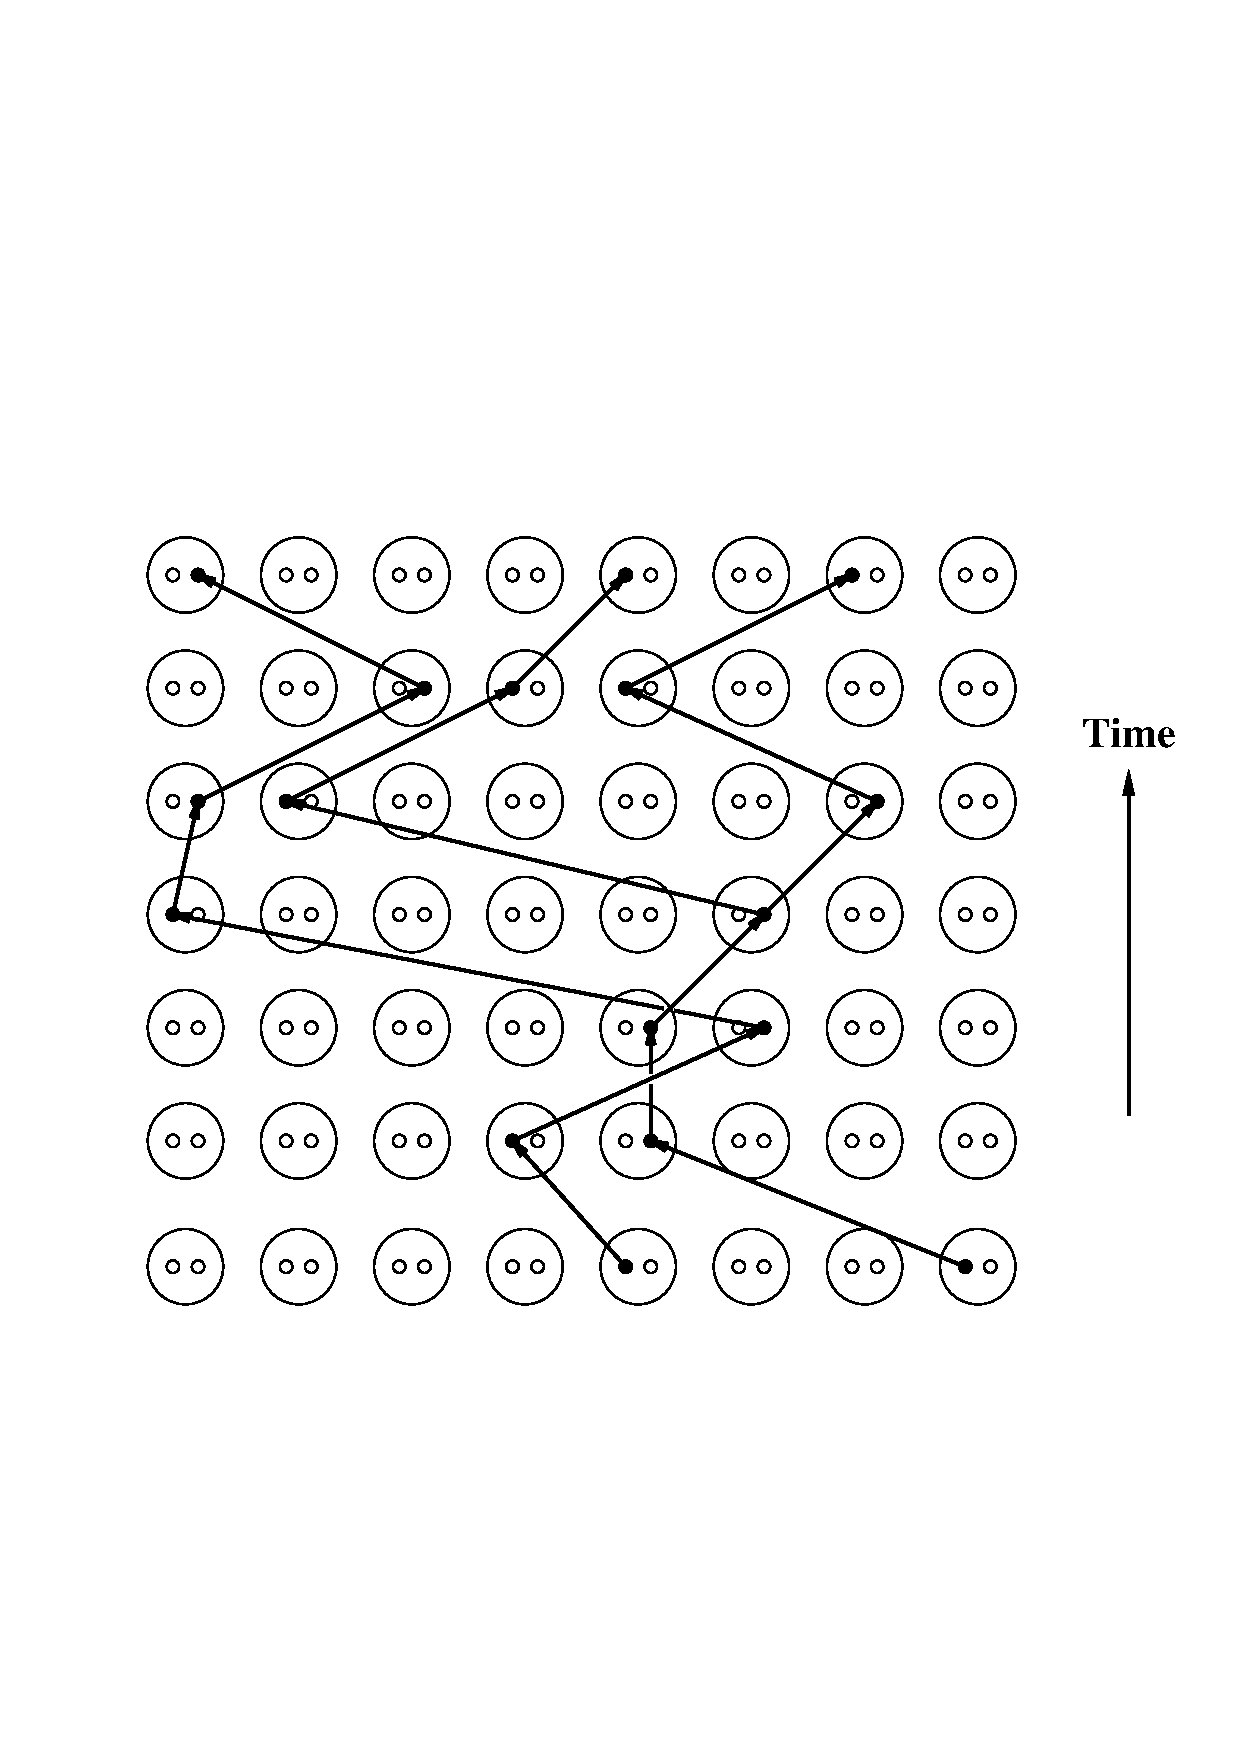
\includegraphics[width=5in]{fig1.pdf}}

\newpage

\centerline{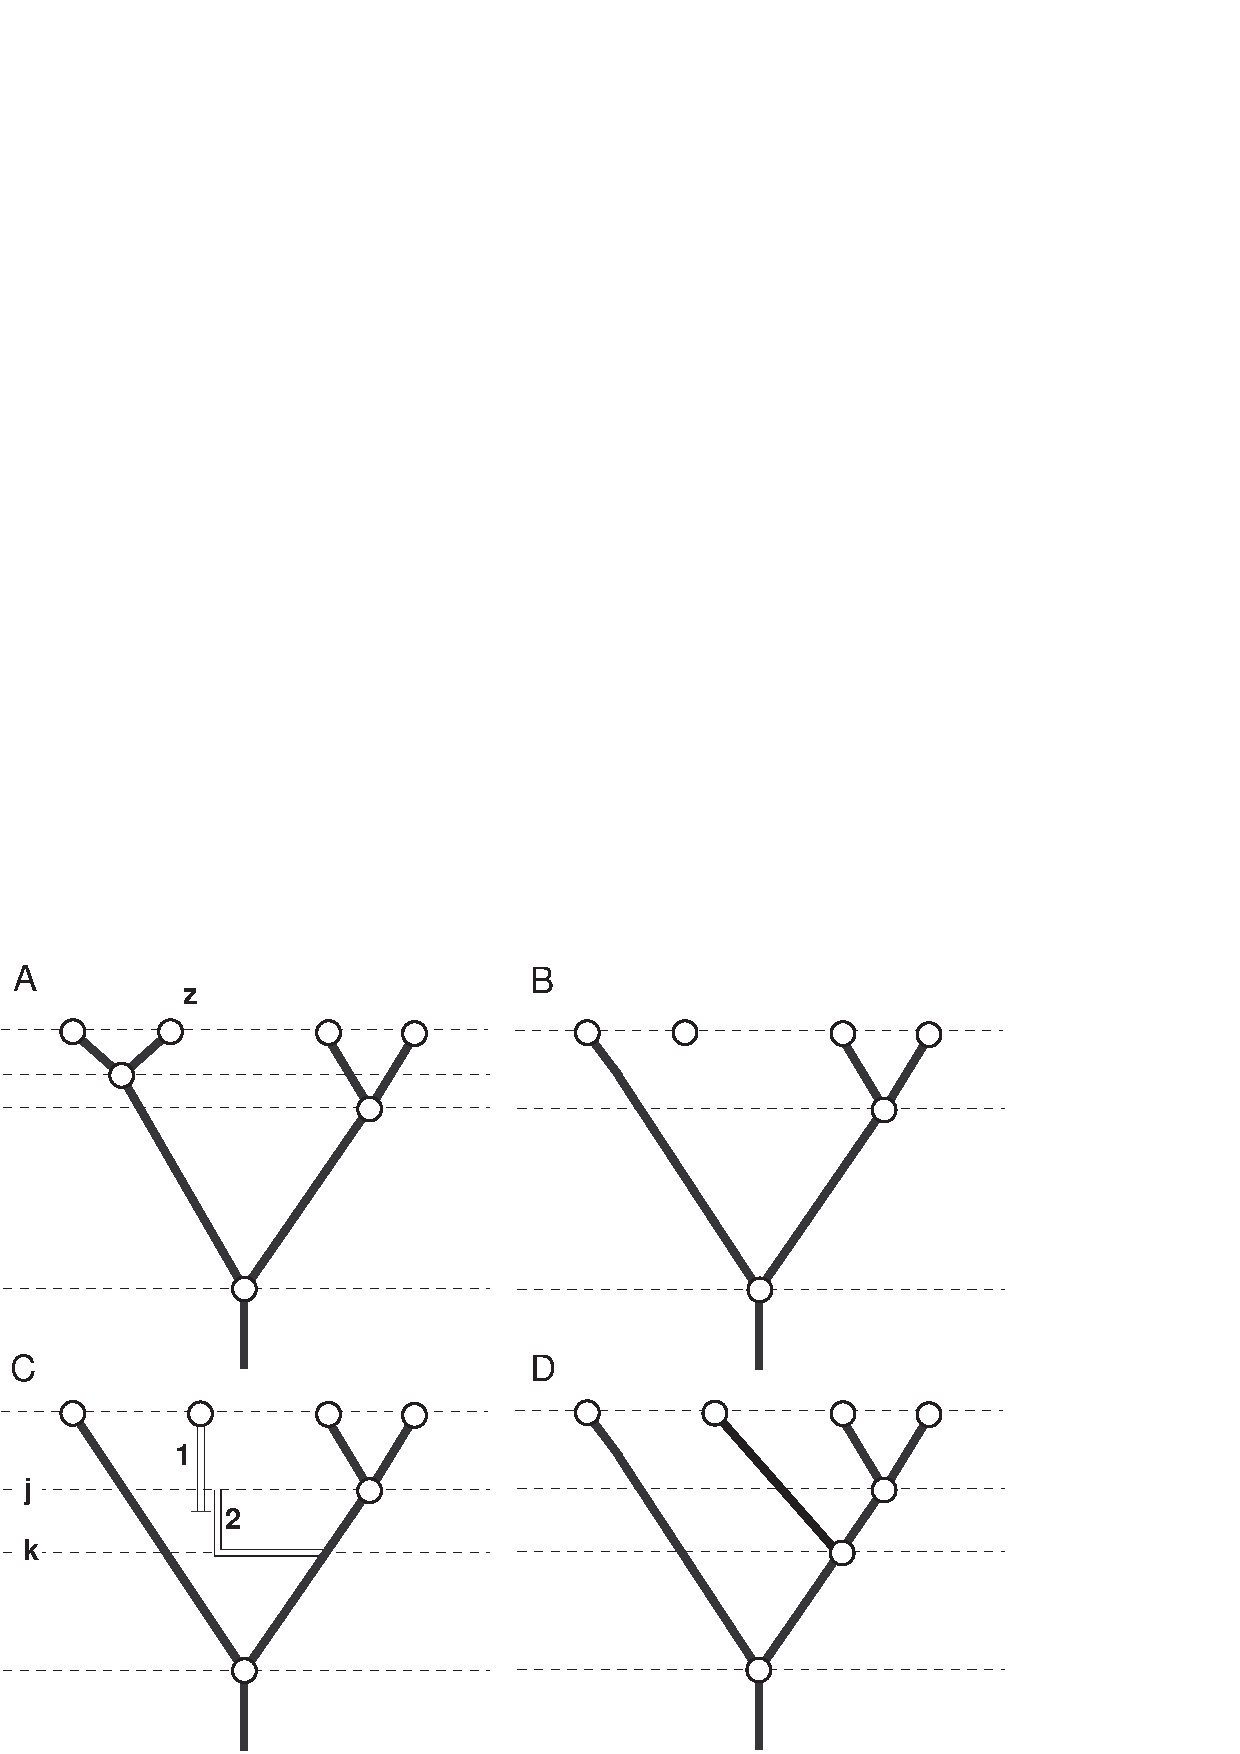
\includegraphics[width=5in]{fig2.pdf}}

\newpage

\centerline{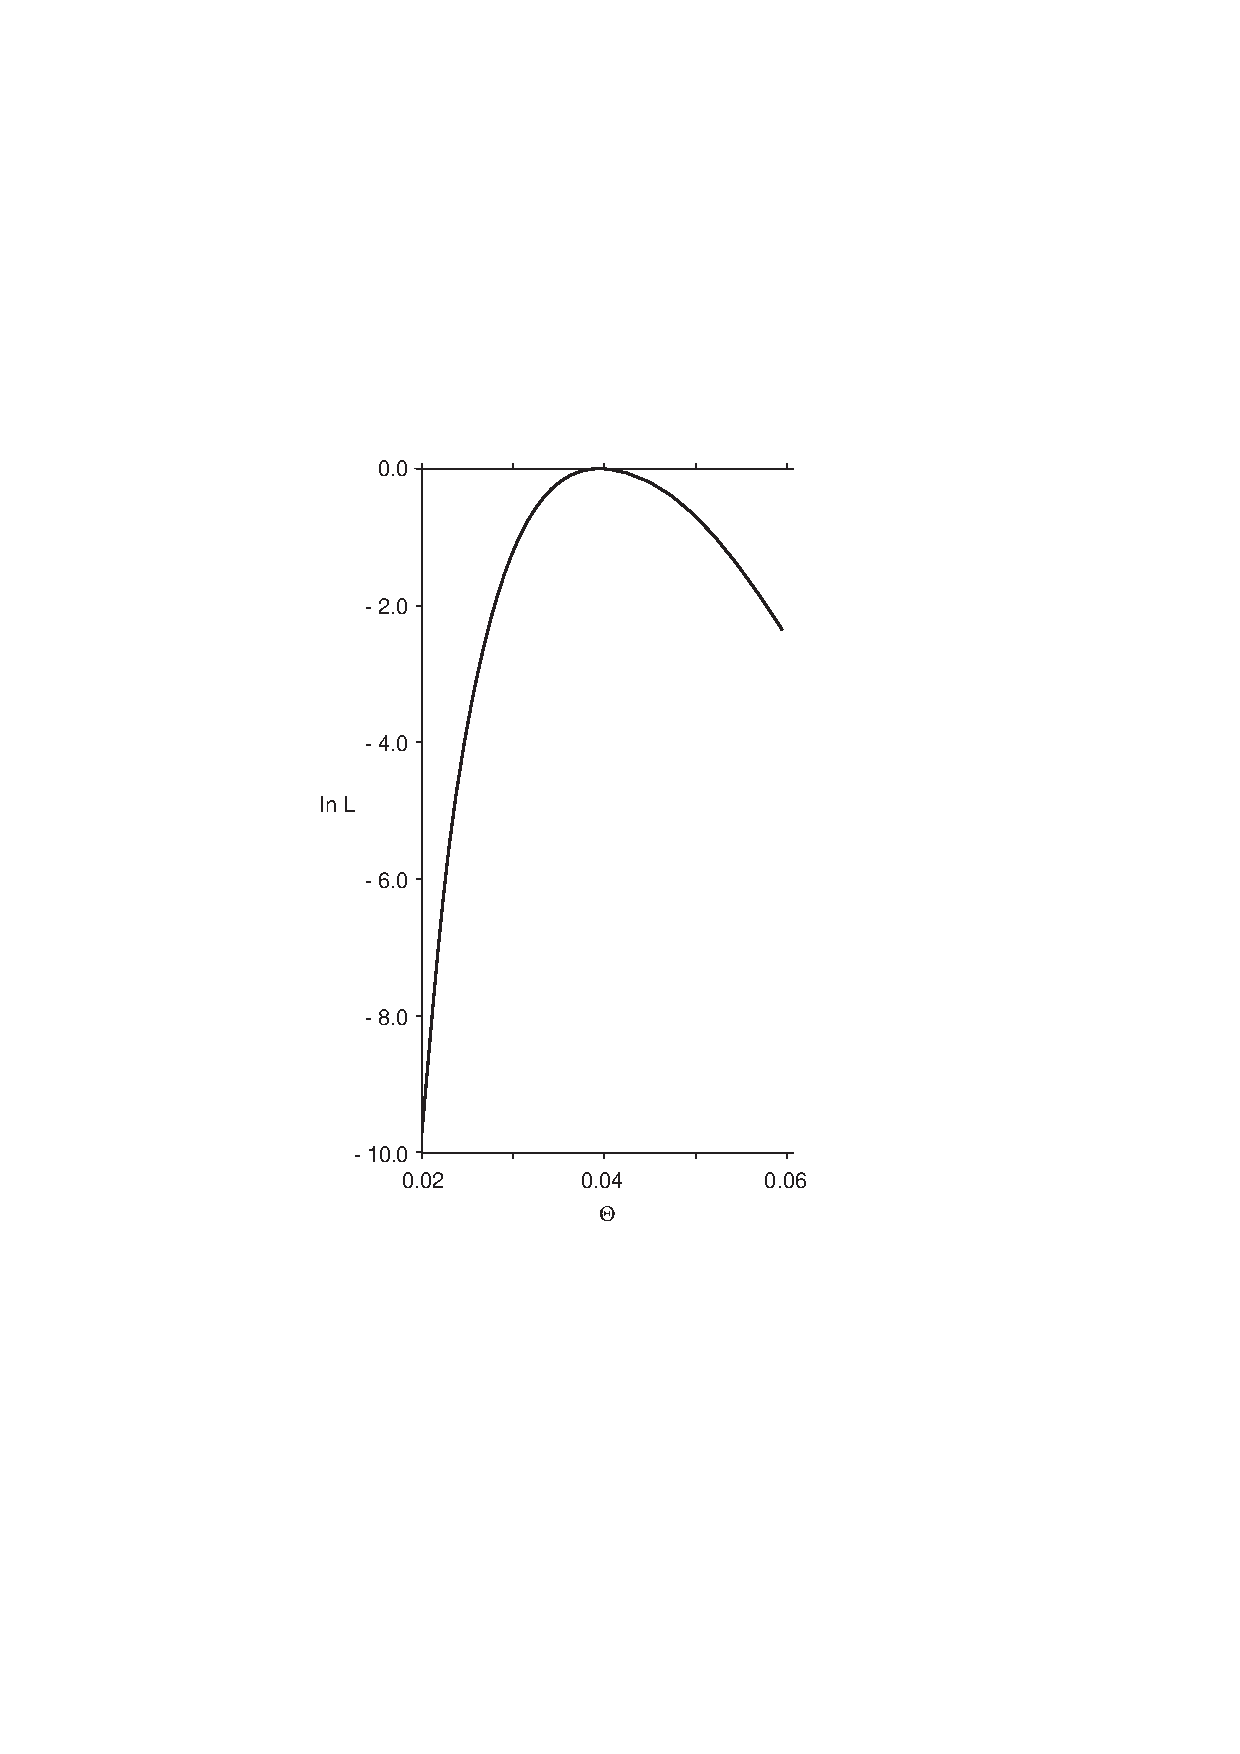
\includegraphics[width=5in]{fig3.pdf}}

\newpage

\centerline{\includegraphics[width=5in]{fig4.pdf}}

\newpage

\centerline{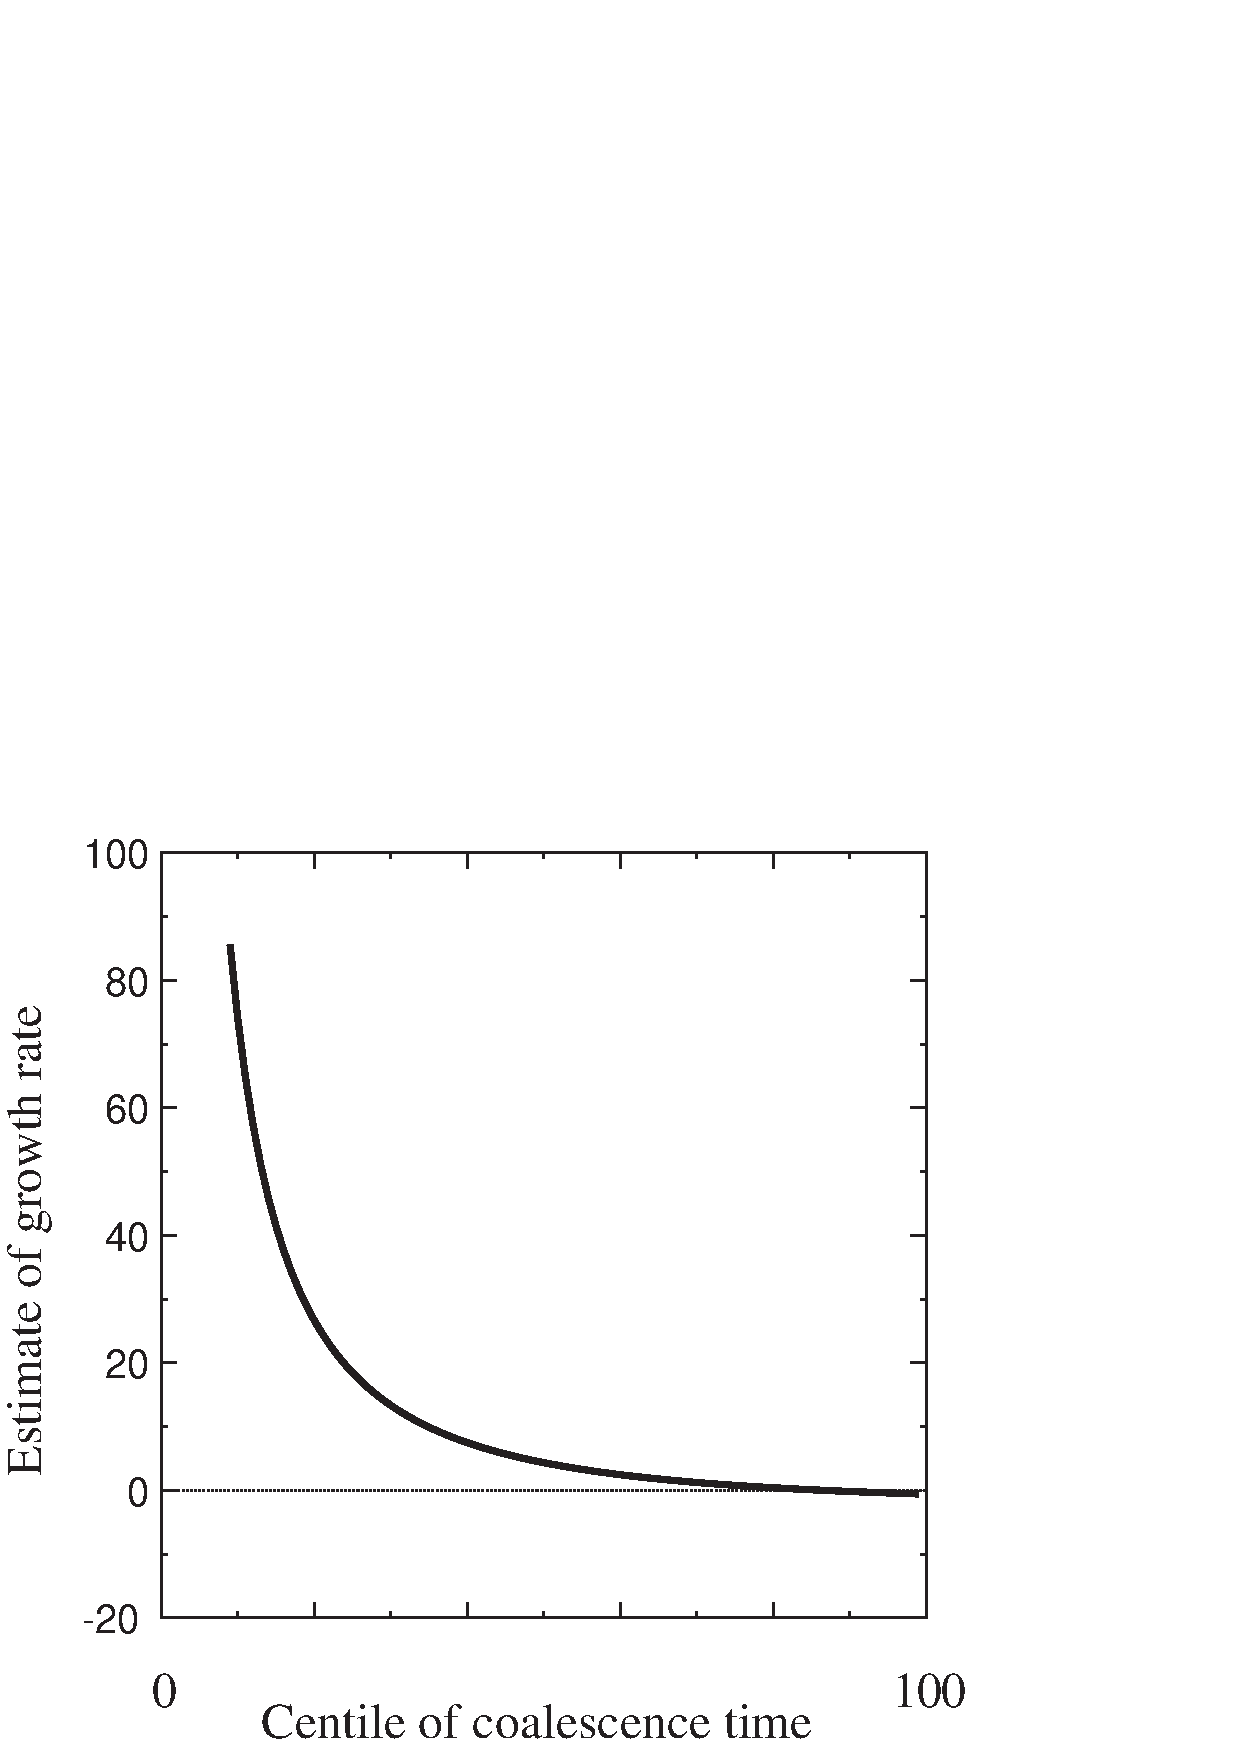
\includegraphics[width=5in]{fig5.pdf}}

\end{document}
